\chapter{The system at a glance}\label{ch:overview}

This book documents every Python file of the \code{tello-balloon-hunter} repository (version 1.0: commit
\code{aab4639}; version 1.1 adds the four safety fixes listed in Appendix~\ref{app:review}). This chapter is the map: what the drone measures, which programs run,
what they send to each other, and in which order to read the rest of the book. Every later chapter goes down
to the level of single functions.

\section{The goal and the hardware}

A DJI Tello (always flown with its protective cage) must fly on its own inside a bedroom, know where it is to a
few centimetres, avoid the furniture, and in the end find and pop balloons. The Tello itself gives us very little:

\begin{center}
\begin{tabular}{@{}lll@{}}
\toprule
Sensor / link & What we get & How we use it \\
\midrule
Front camera & $960\times720$ H.264 video, $\approx 30$ fps, fixed focus & ArUco markers $\Rightarrow$ full 6-DoF pose \\
Downward time-of-flight & \code{tof}: distance to what is below (cm) & height (EKF update), gated over furniture \\
IMU (attitude) & \code{pitch}, \code{roll}, \code{yaw} (deg) & heading update in the EKF (with a learnt offset) \\
Barometer & \code{h}, \code{baro} & \emph{not used}: off by 20 cm at 80 cm \\
Battery & \code{bat} (\%) & takeoff refused below 25\,\%, auto-land at 12\,\% \\
Command link & \code{rc a b c d}, integers in $[-100,100]$ & the only way we move the drone, sent at 20\,Hz \\
\bottomrule
\end{tabular}
\end{center}

The Tello's own downward optical-flow position hold does not work on the plain floor of the room, so the drone
drifts unless \emph{we} hold it. There is no GPS, no motion capture: the only absolute position information is
the camera looking at the markers glued on the walls.

\begin{keypoint}
Everything rests on one idea: the markers' poses in the room are measured once (\file{config/markers.yaml}), so
every time the camera sees a marker, the drone can compute where the camera is. Between two images, and when no
marker is in view, an EKF predicts the motion from the commands we really sent.
\end{keypoint}

\section{The loop in four steps}

\begin{enumerate}[leftmargin=*]
\item \textbf{See the markers} (Chapter~\ref{ch:aruco}). The driver decodes the video and publishes the image;
  \code{aruco\_localizer} detects every marker, solves one joint Perspective-n-Point problem over all their corners
  and publishes the camera-derived drone pose \topic{/aruco/pose}.
\item \textbf{Know where it is all the time} (Chapter~\ref{ch:ekf}). \code{tello\_ekf} fuses that pose (which is
  $\approx 0.5$\,s old when it arrives) with the commands really sent, the distance sensor and the IMU heading,
  and publishes a smooth, delay-compensated state \topic{/ekf/pose}, \topic{/ekf/velocity}, \topic{/ekf/drift}.
\item \textbf{Decide where to go} (Chapter~\ref{ch:missions}). A mission (patrol, strike, marker tour, goto) or the
  keyboard teleop computes a body-frame velocity and sends it on \topic{/tello/cmd\_vel\_safe}.
\item \textbf{Fly safely} (Chapter~\ref{ch:driver}). The driver passes every request through the safety chain
  (climb, position hold, ceiling, height band, flight zone, wall ahead) and sends \code{rc} commands to the Tello.
  What was \emph{really} sent is published on \topic{/tello/rc\_sent}: that is the EKF's input.
\end{enumerate}

Everything the drone needs to know about the room is prepared offline (Chapter~\ref{ch:mapping}): the marker map,
the camera calibration, the 3D scan of the room and the obstacle-free flight zone. The motion model used by the EKF
and the safety layer comes from identification flights (Chapter~\ref{ch:ident}).

\section{ROS 2 in two paragraphs}

A \emph{node} is one program. Nodes exchange typed messages on named \emph{topics} (publish / subscribe, many to
many, asynchronous), call \emph{services} (request / reply, e.g.\ \topic{/tello\_driver/takeoff}), and expose
\emph{parameters} (typed settings, readable by other nodes through the \topic{\textasciitilde/get\_parameters} service:
the missions use it to read the driver's \code{flight\_zone\_file}). The \emph{TF} system is a shared tree of
coordinate frames: anyone can ask ``where is frame A in frame B at time $t$''.

The \emph{QoS} of a topic matters here. Sensor topics use a small queue (\code{depth} 1 for the image) so that a
slow subscriber drops old images instead of accumulating lag. Map-like topics (markers, room mesh, flight zone)
use \emph{transient local} durability: the publisher keeps the last message and hands it to any subscriber that
connects later, which is why RViz shows the room even if it is started after \code{marker\_map\_publisher}.
All nodes run on one laptop, in WSL2, with discovery restricted to localhost
(\file{src/tello\_driver/config/fastdds\_local.xml}).

\section{The node graph}

\begin{figure}[p]
\centering
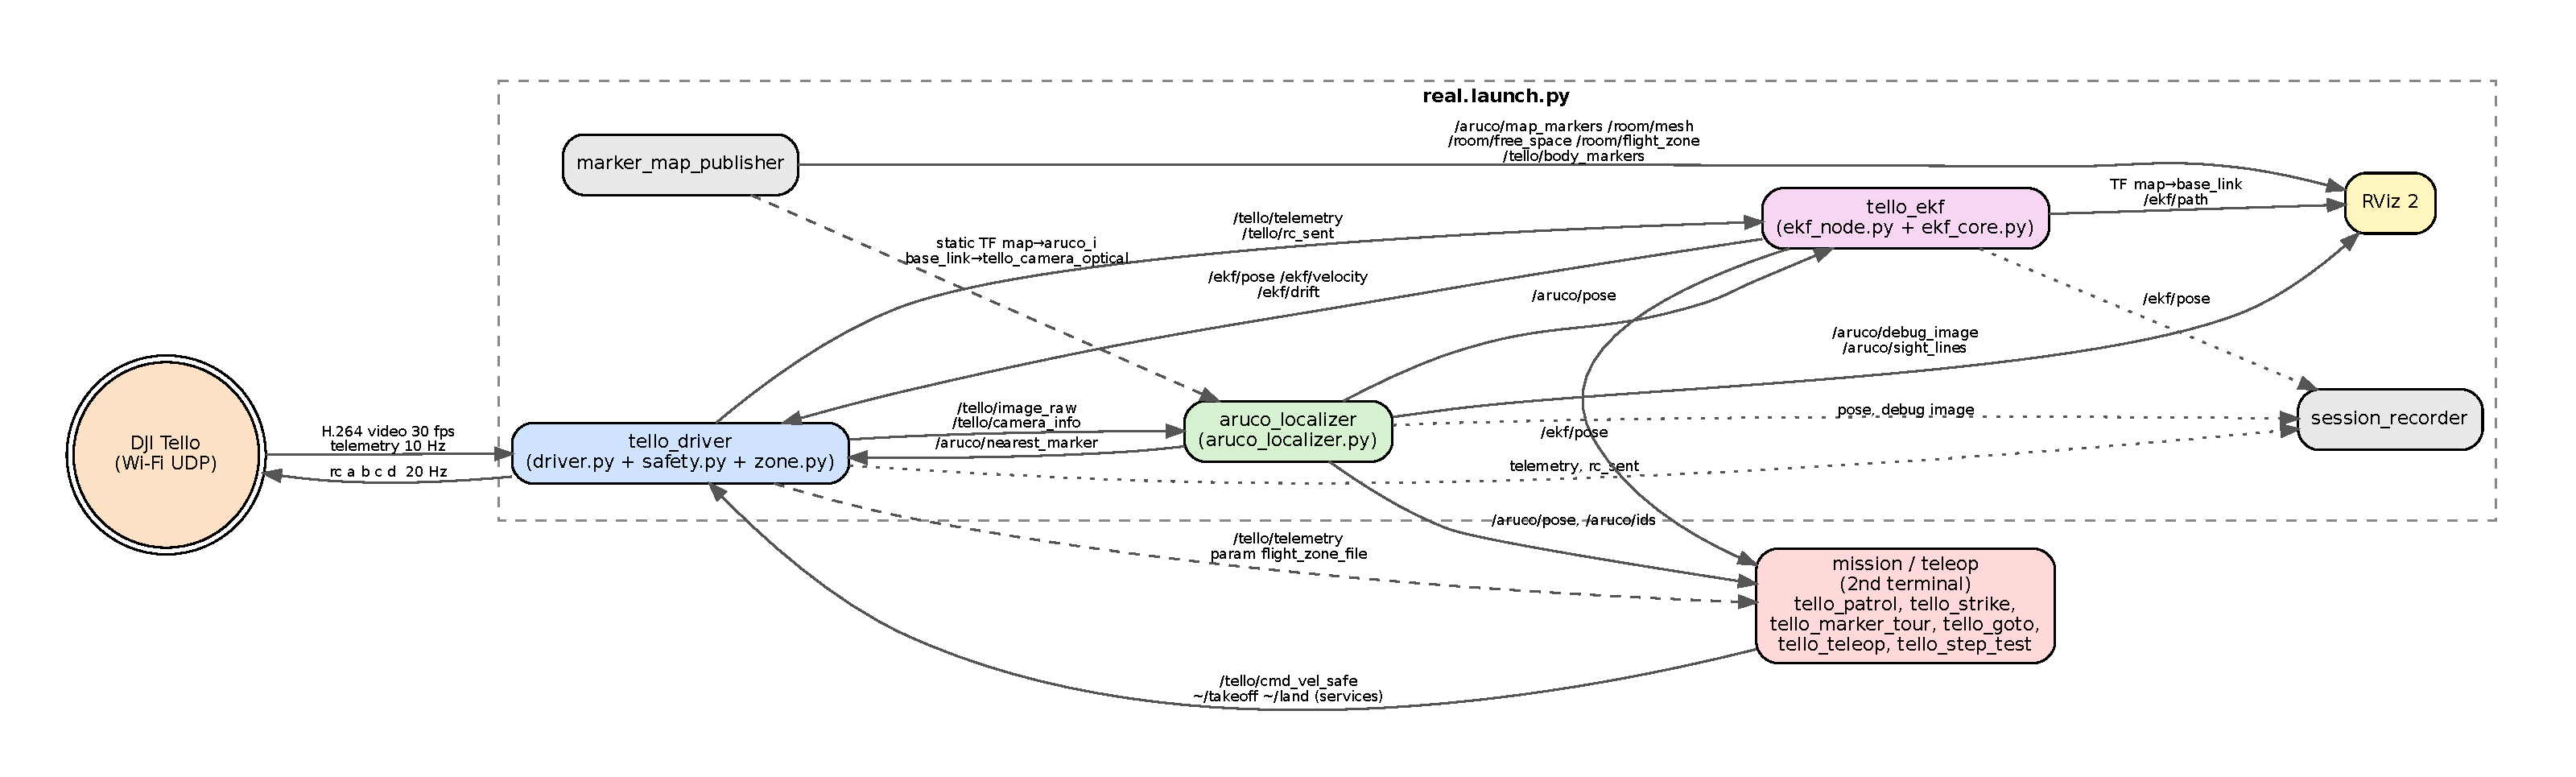
\includegraphics[angle=90,height=0.86\textheight]{figures/ros_graph.pdf}
\caption{Nodes (boxes) and topics (arrows). Dashed: static TF and parameters; dotted: recording only.
Everything inside the dashed frame is started by \file{real.launch.py}; the mission runs in a second terminal.}
\end{figure}

\begin{center}
\small
\begin{longtable}{@{}p{4.2cm}p{3.2cm}p{2.7cm}p{4.6cm}@{}}
\toprule
Topic / service & Type & Publisher & Subscribers \\
\midrule
\endhead
\topic{/tello/image\_raw} & \code{Image} (bgr8) & driver & localizer \\
\topic{/tello/camera\_info} & \code{CameraInfo} & driver & localizer, step\_test \\
\topic{/tello/telemetry} & \code{String} (JSON) & driver & EKF, recorder, teleop, step\_test \\
\topic{/tello/rc\_sent} & \code{Twist} & driver & EKF, recorder, step\_test \\
\topic{/tello/cmd\_vel\_safe} & \code{Twist} & mission / teleop & driver, recorder \\
\topic{/aruco/pose} & \code{PoseWithCovarianceStamped} & localizer & EKF, missions, recorder \\
\topic{/aruco/nearest\_marker} & \code{Float32} (m) & localizer & driver (wall ahead) \\
\topic{/aruco/ids} & \code{String} & localizer & patrol \\
\topic{/aruco/debug\_image} & \code{Image} & localizer & RViz, recorder \\
\topic{/aruco/sight\_lines}, \topic{/aruco/path} & \code{Marker}, \code{Path} & localizer & RViz \\
\topic{/ekf/pose} & \code{PoseWithCovarianceStamped} & EKF & driver, missions, recorder \\
\topic{/ekf/velocity} & \code{TwistStamped} & EKF & driver \\
\topic{/ekf/drift} & \code{Vector3Stamped} & EKF & driver, marker\_tour \\
\topic{/ekf/path} & \code{Path} & EKF & RViz \\
\topic{/aruco/map\_markers} & \code{MarkerArray} & marker\_map\_publisher & RViz \\
\topic{/room/mesh}, \topic{/room/free\_space} & \code{Marker}, \code{OccupancyGrid} & marker\_map\_publisher & RViz \\
\topic{/room/flight\_zone} & \code{MarkerArray} & marker\_map\_publisher & RViz \\
\topic{/tello/body\_markers} & \code{MarkerArray} & marker\_map\_publisher & RViz \\
\topic{/tello\_driver/takeoff}, \topic{land}, \topic{emergency} & \code{Trigger} services & driver & missions, teleop \\
\bottomrule
\end{longtable}
\end{center}

\section{Coordinate frames}

\begin{figure}[h]
\centering
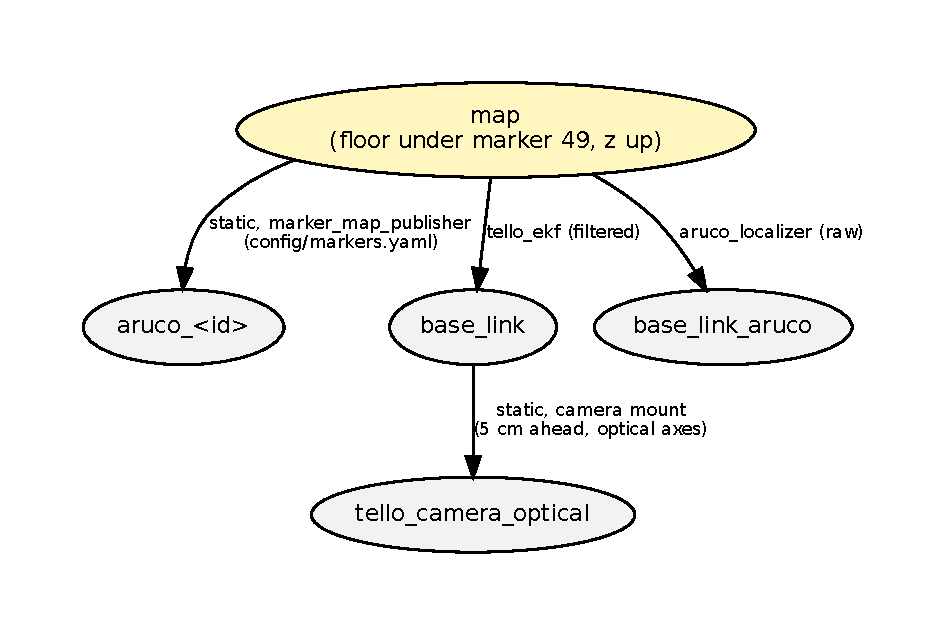
\includegraphics[width=0.62\textwidth]{figures/tf_tree.pdf}
\caption{The TF tree. \code{map} is the room: origin on the floor under marker 49, $z$ up.}
\end{figure}

Two drone frames coexist on purpose: \code{base\_link\_aruco} is the raw, jumpy, $0.5$\,s-old camera pose (useful
to compare), while \code{base\_link} is the EKF estimate that everything else uses. The body convention is the ROS
one ($x$ forward, $y$ left, $z$ up, yaw counter-clockwise); the Tello's \code{rc} convention is
right / forward / up / clockwise, and the driver converts between the two.

\section{The life of one command}

\begin{figure}[h]
\centering
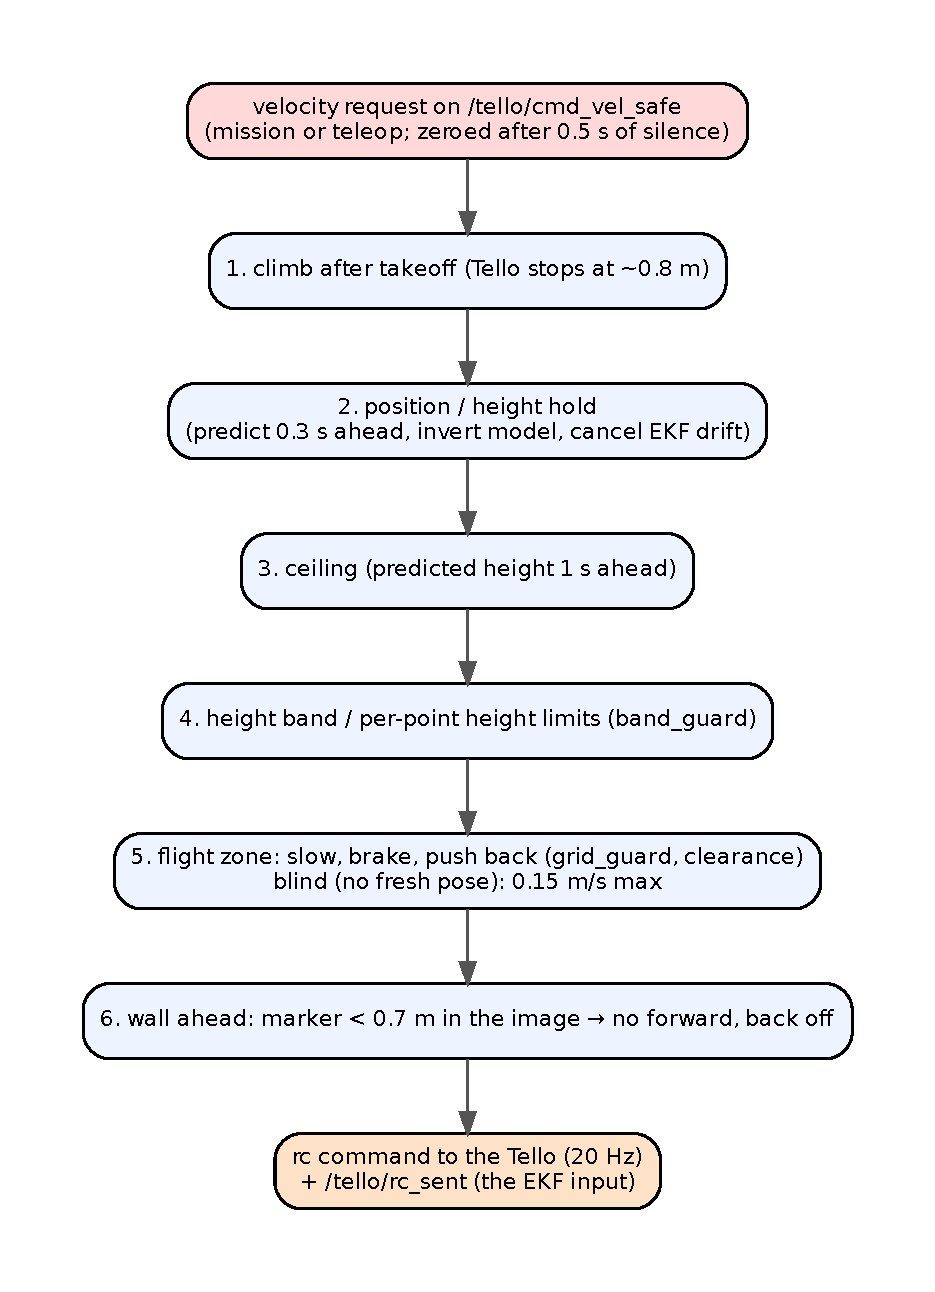
\includegraphics[width=0.66\textwidth]{figures/safety_chain.pdf}
\caption{What the driver does to every velocity request, 20 times per second (Chapter~\ref{ch:driver}).}
\end{figure}

\begin{intuition}
The driver is the \emph{only} node that talks to the drone. That is the reason the safety chain lives there and
not in the missions: whatever program asks for a velocity (a mission with a bug, the keyboard, a future balloon
attack), the request passes through the same checks. Missions are free to be simple and aggressive; the driver
says no. Conversely, the driver contains no mission logic: it does not know what a marker tour or a balloon is.
\end{intuition}

\section{Timing and latency}

\begin{center}
\begin{tabular}{@{}lr@{}}
\toprule
Step & Typical delay \\
\midrule
\code{rc} command $\to$ the drone starts to move ($L_u$) & $0.35$\,s \\
Image exposure $\to$ \topic{/aruco/pose} published ($L_v$) & $0.20$\,s \\
Command $\to$ its effect is seen in a marker pose ($L_u+L_v$) & $0.55$\,s \\
Driver control loop & 20\,Hz \\
Marker poses (markers in view) & $\approx 20$ poses/s \\
\bottomrule
\end{tabular}
\end{center}

A delay of more than half a second is enormous for a drone flying at $0.3$--$0.5$\,m/s: it has moved $15$--$25$\,cm before
we see it. This is why the EKF applies each pose \emph{at the time the image was taken} and re-propagates to now,
and why the position hold predicts $0.3$\,s ahead. The identified model per horizontal axis is
\begin{equation*}
\tau\,\dot v(t) = K\,u(t-L_u) - v(t), \qquad K_x = 0.66,\quad K_y = 0.83,\quad \tau = 0.25\text{ s},\quad L_u = 0.35\text{ s},
\end{equation*}
identified with the cage on November 13 (\file{core/model.py}, Chapter~\ref{ch:ident}). $K<1$: the caged drone flies
slower than the \code{rc} gain promises.

\section{The offline pipeline}

\begin{figure}[h]
\centering
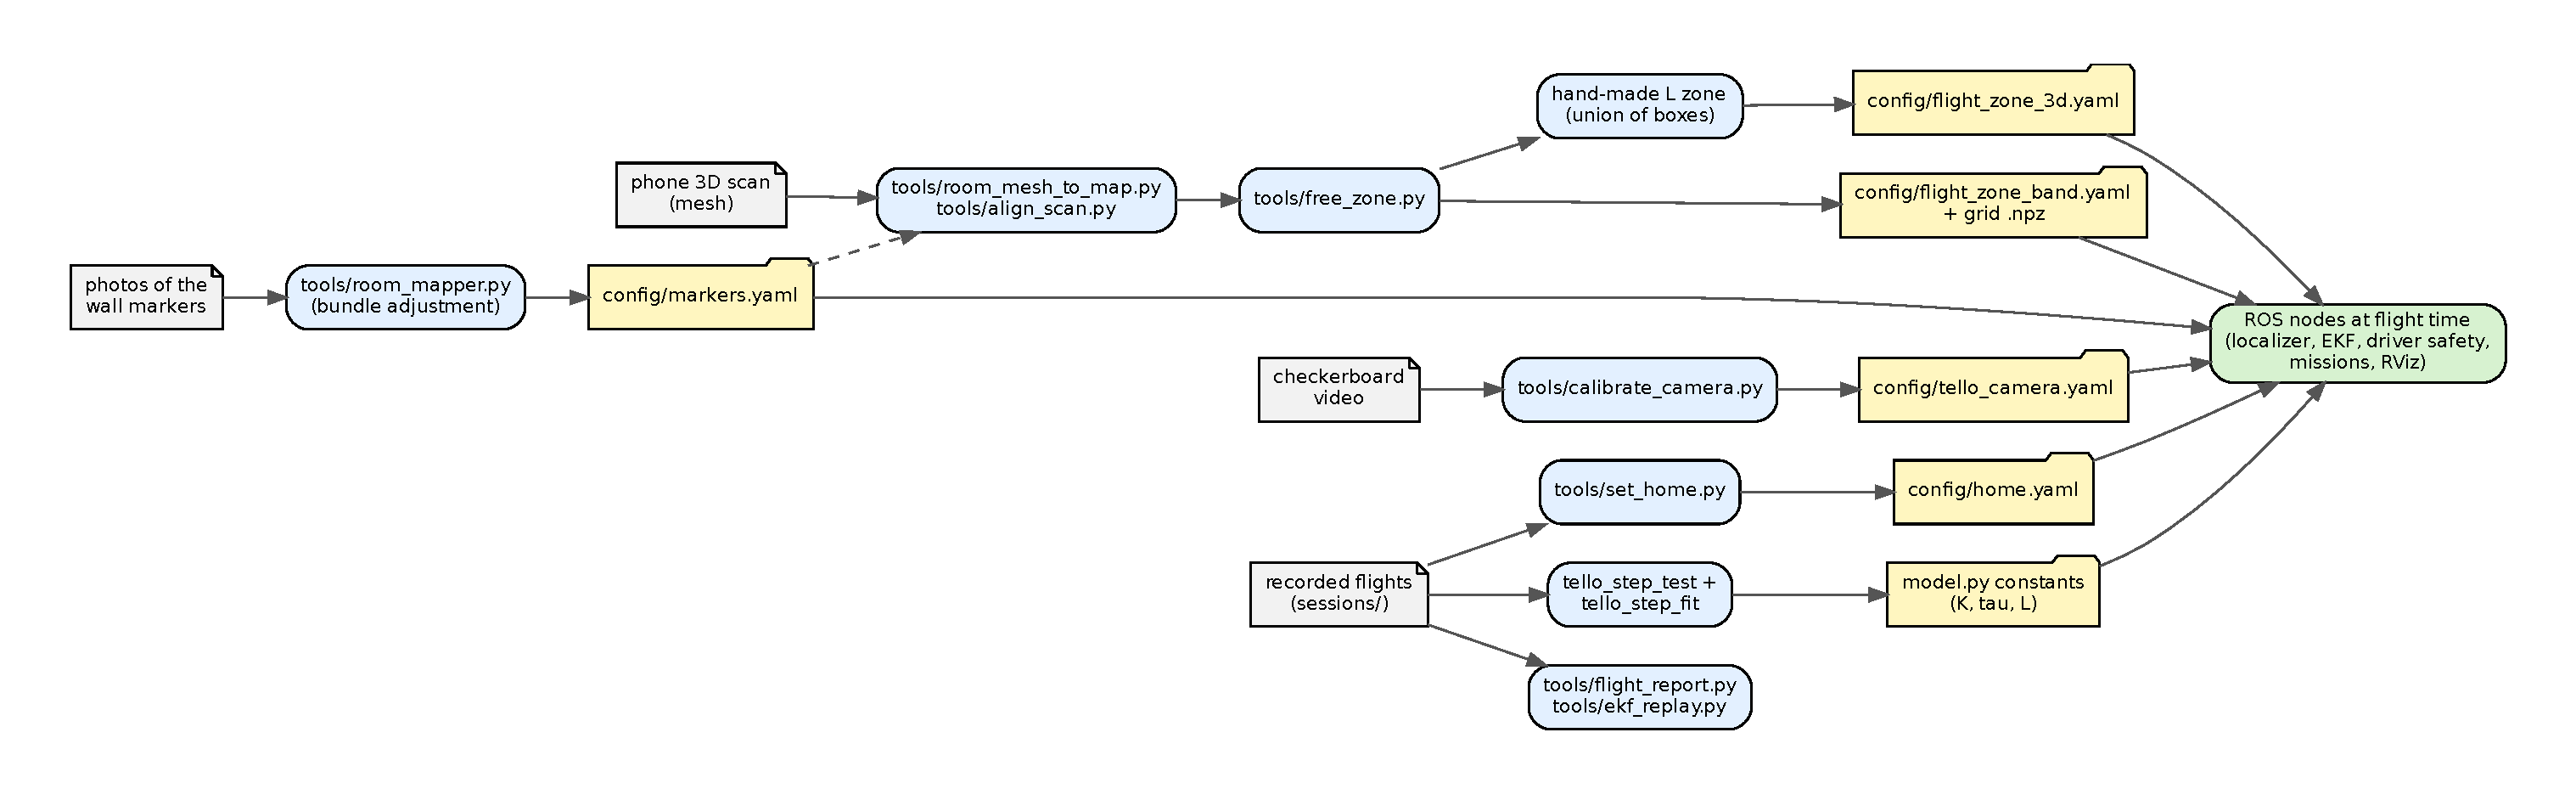
\includegraphics[width=\textwidth]{figures/offline.pdf}
\caption{Everything prepared before a flight, and the files it produces.}
\end{figure}

\section{Package layout: why each file exists}\label{sec:layout}

Since November 19 the ROS package \file{tello\_driver} is split by \emph{when the code runs}: \file{core/} runs on
every flight, whatever the mission; \file{missions/} holds the flight programs; \file{identification/} measures the
model they all use; \file{sim/} replaces the drone in tests. The executable names (\code{ros2 run tello\_driver
...}) did not change. Every \file{\_\_init\_\_.py} repeats this list in its docstring.
Chapter~\ref{ch:safetylayer} then separates, inside these files, the nominal pipeline from the safety layer.

\begin{center}
\small
\begin{longtable}{@{}p{5.2cm}p{8.4cm}c@{}}
\toprule
File & Why it exists & Ch. \\
\midrule
\endhead
\multicolumn{3}{@{}l}{\textbf{\file{src/aruco\_localization/aruco\_localization/}}: camera $\to$ pose} \\
\file{aruco\_localizer.py} & marker detection, joint PnP, \topic{/aruco/pose} & \ref{ch:aruco} \\
\file{marker\_map.py} & loads \file{markers.yaml}, marker corner geometry (also used by the tools) & \ref{ch:aruco} \\
\file{marker\_map\_publisher.py} & static TFs, RViz room / zone / markers & \ref{ch:aruco} \\
\midrule
\multicolumn{3}{@{}l}{\textbf{\file{src/tello\_driver/tello\_driver/core/}}: runs on every flight} \\
\file{driver.py} & the only node that talks to the Tello: video, telemetry, services, 20\,Hz \code{rc}; camera and link failsafe & \ref{ch:driver} \\
\file{safety.py} & \code{CommandFilter}: hold, ceiling, band, zone, wall guards on every command & \ref{ch:driver} \\
\file{zone.py} & flight zone, clearance grids, 3D boxes & \ref{ch:driver} \\
\file{ekf\_core.py} & the EKF, pure numpy (also replayed offline by \file{tools/ekf\_replay.py}) & \ref{ch:ekf} \\
\file{ekf\_node.py} & its ROS wrapper: \topic{/aruco/pose} + \topic{/tello/rc\_sent} in, \topic{/ekf/pose} out & \ref{ch:ekf} \\
\file{model.py} & the identified constants $K$, $\tau$, $L_u$, shared by EKF, guards, missions, sim & \ref{ch:ekf} \\
\file{home.py} & the takeoff pad, for the return before landing & \ref{ch:missions} \\
\file{video\_reader.py} & optional low-latency H.264 decoding (\code{low\_latency\_video:=true}) & \ref{ch:driver} \\
\file{ros\_env.py} & local-only DDS settings for every node & \ref{ch:driver} \\
\file{session\_recorder.py} & flight logs (video, poses, commands) & \ref{ch:ident} \\
\file{teleop.py} & keyboard flight; its \code{read\_key} is the ``any key = land'' of the missions & \ref{ch:missions} \\
\midrule
\multicolumn{3}{@{}l}{\textbf{\file{missions/}}: flight programs} \\
\file{base.py} & \code{Mission}: inputs, takeoff, start point, safety checks, 20\,Hz loop, search, logs & \ref{ch:missions} \\
\file{tour.py} & \code{goto} in front of a marker; \code{tello\_marker\_tour} and \code{tello\_goto 49 35} & \ref{ch:missions} \\
\file{patrol.py} & laps of the zone, type a marker id to go to it & \ref{ch:missions} \\
\file{strike.py}, \file{trajectory.py} & fast planned legs with model feedforward (quintic trajectories) & \ref{ch:missions} \\
\midrule
\multicolumn{3}{@{}l}{\textbf{\file{identification/}}: where \file{core/model.py} comes from} \\
\file{step\_test.py} & identification / validation flight (velocity doublets), a \code{Mission} on the raw pose & \ref{ch:ident} \\
\file{step\_fit.py} & fits gain, time constant and delay per axis $\to$ \file{model.yaml} & \ref{ch:ident} \\
\midrule
\multicolumn{3}{@{}l}{\textbf{\file{sim/}}: tests without hardware (\code{mock:=true})} \\
\file{fake\_tello.py} & same interface as djitellopy's \code{Tello}; \code{FAKE\_VIDEO\_OFF} cuts its video & \ref{ch:driver} \\
\file{fake\_world.py} & identified dynamics + rendered camera view of the marker map & \ref{ch:driver} \\
\midrule
\multicolumn{3}{@{}l}{\textbf{\file{tools/}} (offline, run by hand) and launch} \\
\file{flight\_report.py}, \file{ekf\_replay.py},\newline \file{calibrate\_camera.py}, \file{make\_print\_sheets.py} & analysis, EKF replay, calibration, printing & \ref{ch:ident} \\
\file{room\_mapper.py}, \file{align\_scan.py},\newline \file{room\_mesh\_to\_map.py} & marker map, room scan & \ref{ch:mapping} \\
\file{free\_zone.py}, \file{zone\_view.py}, \file{set\_home.py} & flight zone, viewer, takeoff pad & \ref{ch:mapping} \\
\file{ext\_camera.py} & external camera: self-calibration on the wall markers, balloons in the map (Windows side) & --- \\
\file{tello\_driver/launch/}\newline\file{real.launch.py}, \file{tello.bat} & starting everything & \ref{ch:mapping} \\
\bottomrule
\end{longtable}
\end{center}

\section{How to run it}

\begin{lstlisting}[language=bash]
# terminal 1 (WSL): driver + localizer + EKF + marker map + RViz
ros2 launch tello_driver real.launch.py                 # band zone (default)
ros2 launch tello_driver real.launch.py flight_zone:=3d # the L-shaped 3D zone
ros2 launch tello_driver real.launch.py mock:=true      # simulated drone
# terminal 2: a mission or the keyboard
ros2 run tello_driver tello_patrol      # laps; type 35 + ENTER = go to marker 35
ros2 run tello_driver tello_teleop
\end{lstlisting}
Or double-click \file{tello.bat} on Windows, which connects the Wi-Fi dongle to the drone and opens both terminals.
